\documentclass{report}
\usepackage{graphicx}
\usepackage{float}

\setcounter{tocdepth}{4}

\usepackage[pdfborder={0 0 0}]{hyperref}
\usepackage{wrapfig}
\begin{document}

\section{Initial Condition Generation}
We first had to generate the initial positions of the stars a galaxy. Galaxies have several properties we must take into account:
\begin{enumerate}
  \item Shape of the spiral arms and central bulge. 
  \item The density of the stars
  \item The velocity of the stars 
  \item The distribution of the dark matter. 
\end{enumerate}
\subsubsection{Shape and Density of the Arms and Central Bulge}
In a standard spiral galaxy the arms have the shape of a logeritmic spiral -CITE-. There are several models as to why the spiral arms have the shape they do. For this project we used the spiral density waves theory firs developed by C. C. Lin and Frank Shu in 1964 -CITE-. In this model stars have elliptical orbits and that the size and rotation of theses ellipse varied in a correlated way. Figure \ref{fig:spiral-arms} shows an example of this.
\begin{figure}
\centering
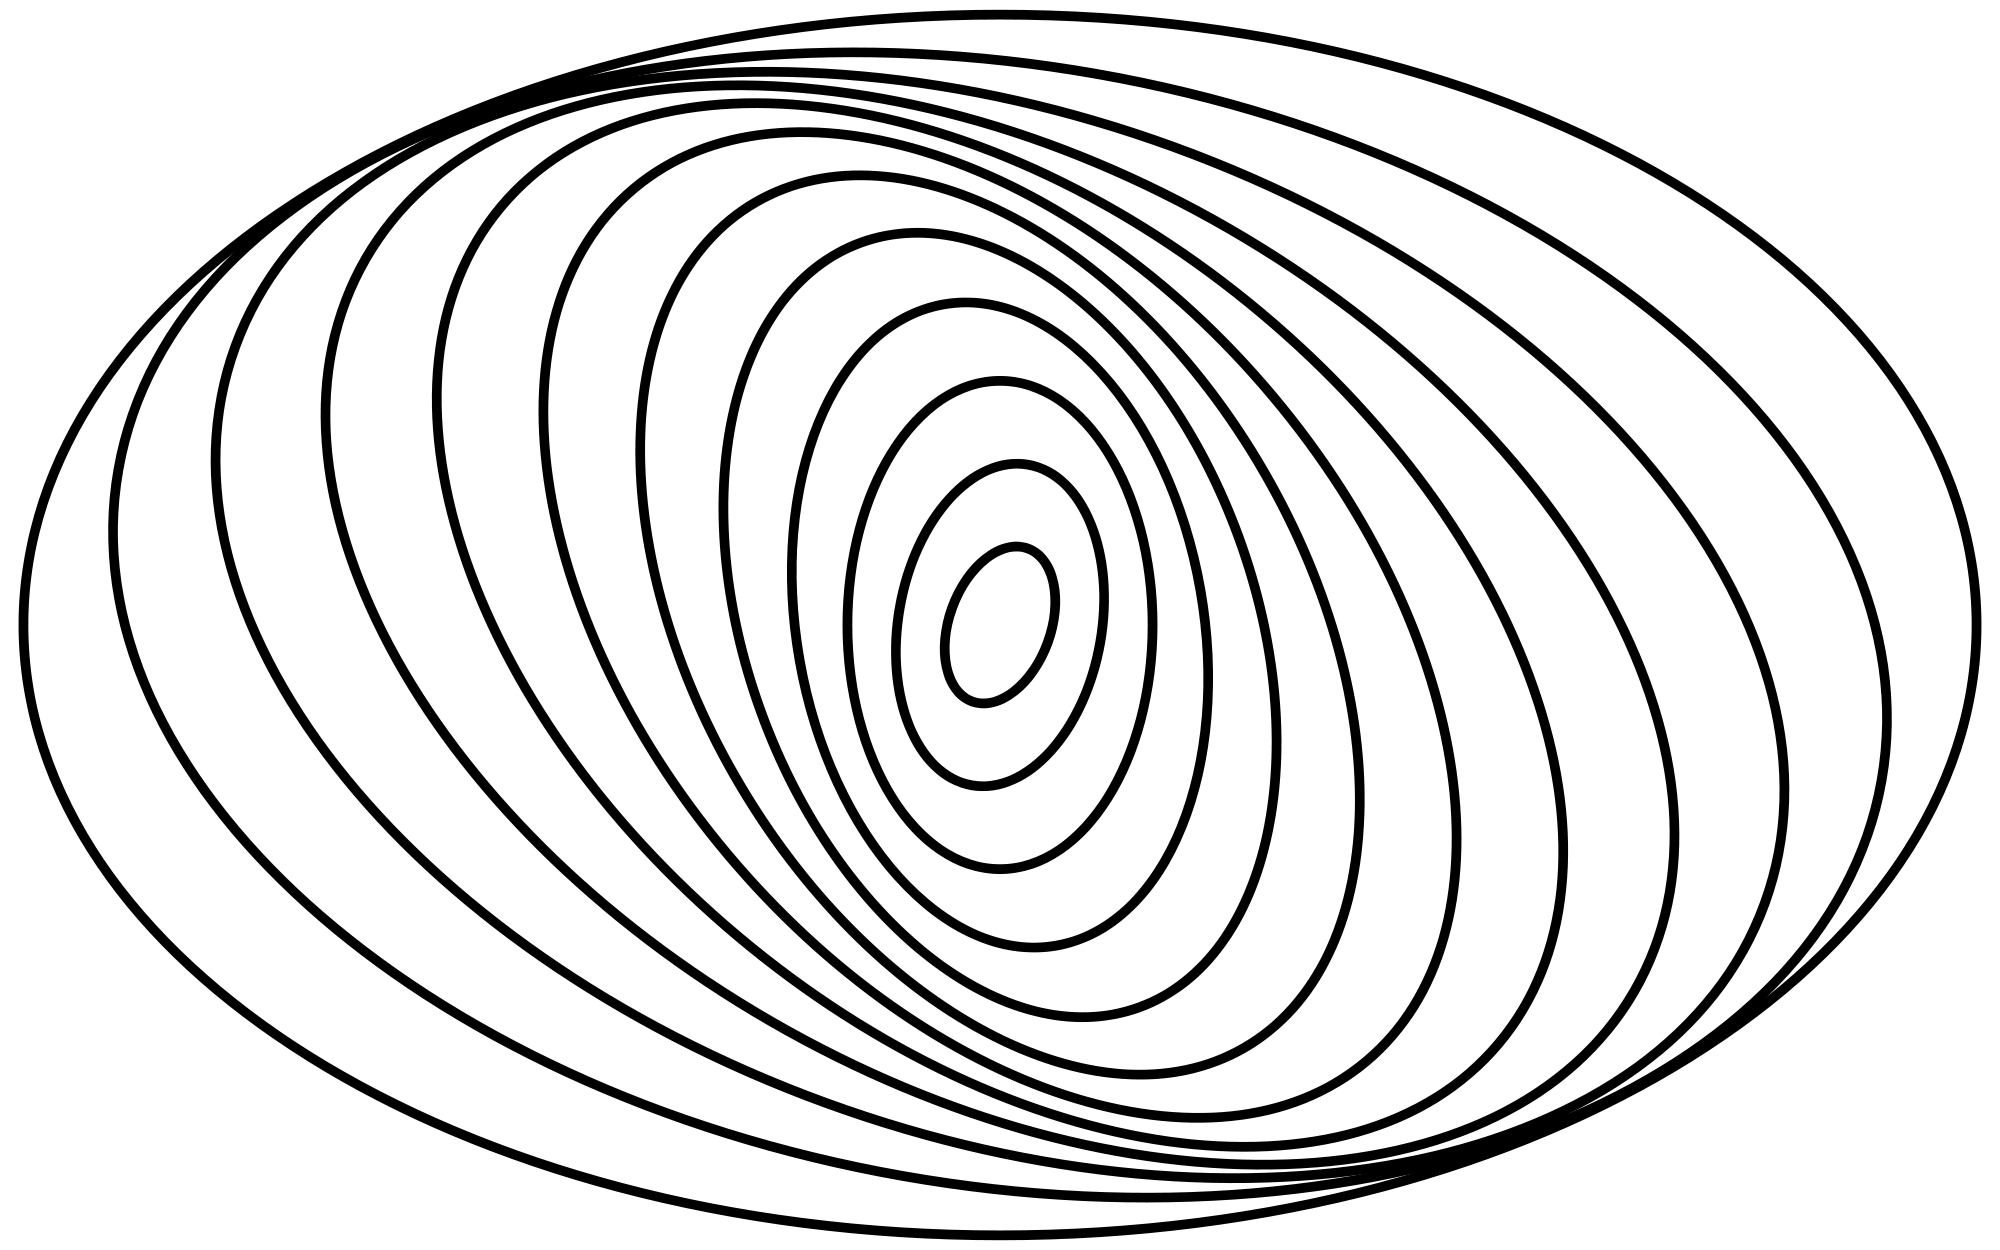
\includegraphics[width=.8\columnwidth]{spiral-arms.png}
\caption{An explanation of spiral galaxy arms.  The ellipses are stars' orbits around the galactic center.  The arms are areas of high density. \label{fig:spiral-arms}}
\end{figure}

The density of stars in a spiral galaxy goes off as $e^{-r}$ -CITE-. To generate a distribution that fit this model we created a list of ellipses, in the form of a parametric equation, that fit the model above where the density of ellipses went as $e^{-r}$. Then each ellipse was filled with the same number stars, at a random location along the ellipse. Each location was then slightly randomized. The z component was then fit to a normal distribution about the x-y plane. 

Around the center of a normal spiral galaxy there is a central bulge. We approximated this with a constant density sphere around the origin. 

\subsubsection{Velocities}
\begin{figure}
\centering
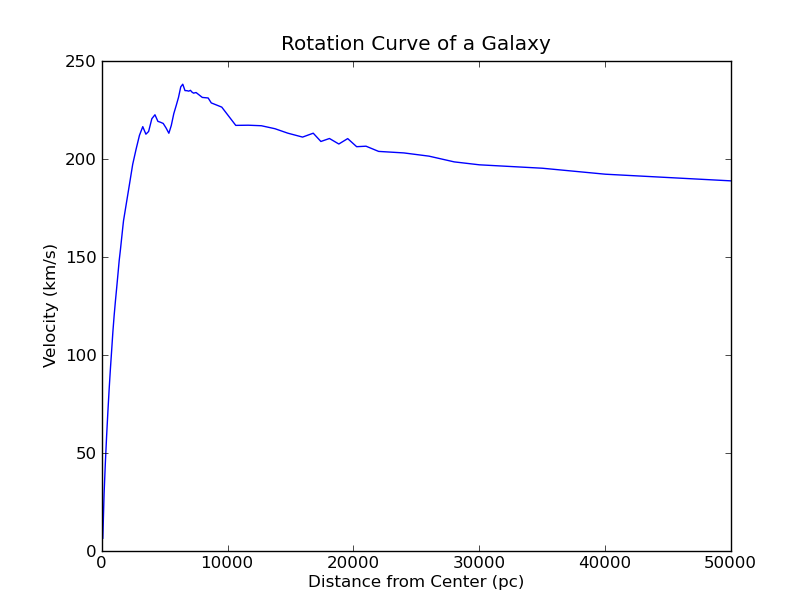
\includegraphics[width=.8\columnwidth]{rotation_curve.png}
\caption{The rotation curve we fit our initial velocities to. -CITE- } 
\label{fig:vel}
\end{figure}
To find the velocities of the stars we fit the velocities to a measured rotation curve -CITE- Figure \ref{fig:vel} shows the data we fit to. The velocities in the spiral arms were then pointed along the direction of the ellipse, with a small random component. For the central bulge we had the orbits be circular around the origin but in a random plane. 
\subsubsection{Dark Matter}
\begin{figure}[H]
 \centering
 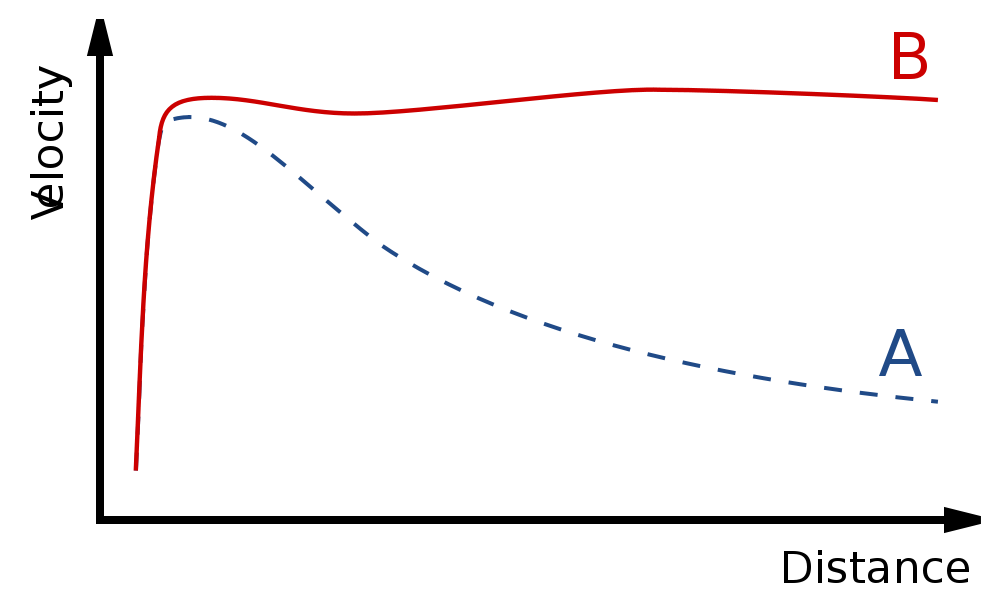
\includegraphics[width=0.5\textwidth]{./rotation.png}
  \caption{The rotation curve of the stars in a typical spiral galaxy. Curve A is the results predicted by
 Newtonian mechanics. Curve B is the observed results. Source:  \url{http://en.wikipedia.org/wiki/Galaxy_rotation_curve} } 
 \label{fig:rot}
\end{figure}

Figure \ref{fig:rot} shows evidence for the presence of dark matter in a typical galaxy. The rotation curve of the stars in a typical spiral galaxy. Curve A is the results predicted by
 Newtonian mechanics. Curve B is the observed results. We also must include dark matter if we want our galaxy to be stable. We choose a spherical, constant density halo distribution of dark matter around the galaxy. Figure \ref{fig:dark} shows an example of a distribution we used. The actual distribution was dense, it was thinned out for clarity.

\begin{figure}[H]
 \centering
 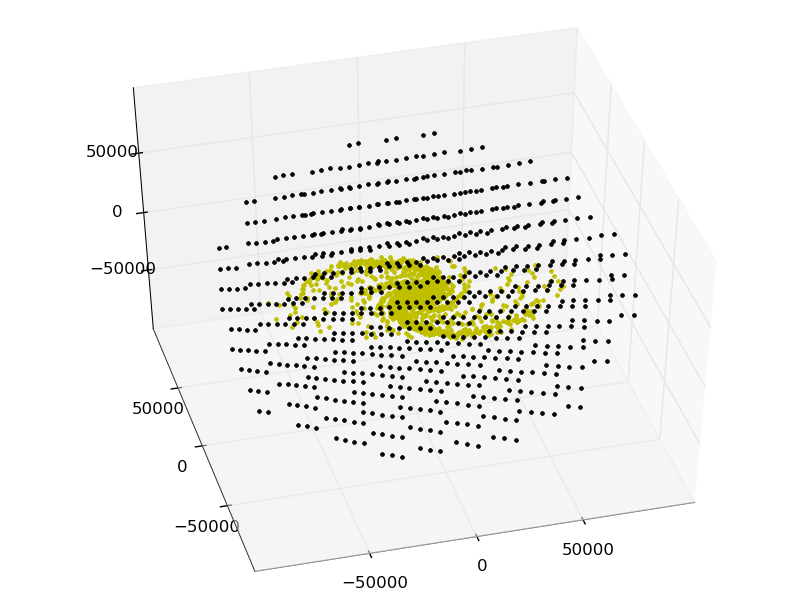
\includegraphics[width=\textwidth]{./darkmatterdist.png}
  \caption{Shows a version of the dark matter distribution we used. The actual distribution was dense, it was thinned out for clarity. } 
 \label{fig:dark}
\end{figure}



 
\end{document}
